

\documentclass{acm_proc_article-sp}


\usepackage{graphicx}
\usepackage{listing}
\usepackage{listings} \lstset{basicstyle=\tiny,numbers=none, breaklines=true, numberstyle=\tiny, numbersep=5pt,firstnumber=last,language=XML,escapeinside={(*@}{@*)} }  

% *** CITATION PACKAGES ***
%
\usepackage{cite}
\usepackage{url}
%\usepackage[scaled=point85]{luximono}
\hyphenation{op-tical net-works semi-conduc-tor name-space}

\begin{document}

\title{VIENNA Add-In \\ Visualizing Inter-ENterprise Network Architectures}


\numberofauthors{2} %  in this sample file, there are a *total*
% of EIGHT authors. SIX appear on the 'first-page' (for formatting
% reasons) and the remaining two appear in the \additionalauthors section.
%
\author{
% You can go ahead and credit any number of authors here,
% e.g. one 'row of three' or two rows (consisting of one row of three
% and a second row of one, two or three).
%
% The command \alignauthor (no curly braces needed) should
% precede each author name, affiliation/snail-mail address and
% e-mail address. Additionally, tag each line of
% affiliation/address with \affaddr, and tag the
% e-mail address with \email.
%
% 1st. author
\alignauthor
Christian Huemer, Philipp Liegl, Thomas Motal, Rainer Schuster, Marco Zapletal \\
       \affaddr{Vienna University of Technology}\\
       \affaddr{Favoritenstrasse 9-11/188}\\
       \affaddr{1040 Vienna, Austria}\\
       \email{\{firstname.lastname\}@tuwien.ac.at}       
\alignauthor
Christian Eis, Martina Hiesinger, Fabian Kromer, Robert Kromer, Andreas Kuntner, Christian Pichler, Michael Strommer\\
       \affaddr{Research Studios Austria}\\
       \affaddr{Thurngasse 8/3/20}\\
       \affaddr{1090 Vienna, Austria}\\
       \email{office.ios@researchstudio.at}       
% 2nd. author
%\alignauthor
%Christian Pichler\\
%       \affaddr{Research Studios Austria}\\
%       \affaddr{Thurngasse 8/3/20}\\
%       \affaddr{1090 Vienna, Austria}\\
%       \email{cpichler@researchstudio.at}
}

\date{28 April 2009}

\maketitle
\begin{abstract}



\end{abstract}

% A category with the (minimum) three required fields
\category{H.4}{Information Systems Applications}{Miscellaneous}


\terms{Business document modeling, conceptual modeling, XML schema generation}




\section{Introduction} by PL

- explain the use case scenario of the add-in

- motivate the model driven approach for SOA artifacts


\begin{figure}
 \centering
   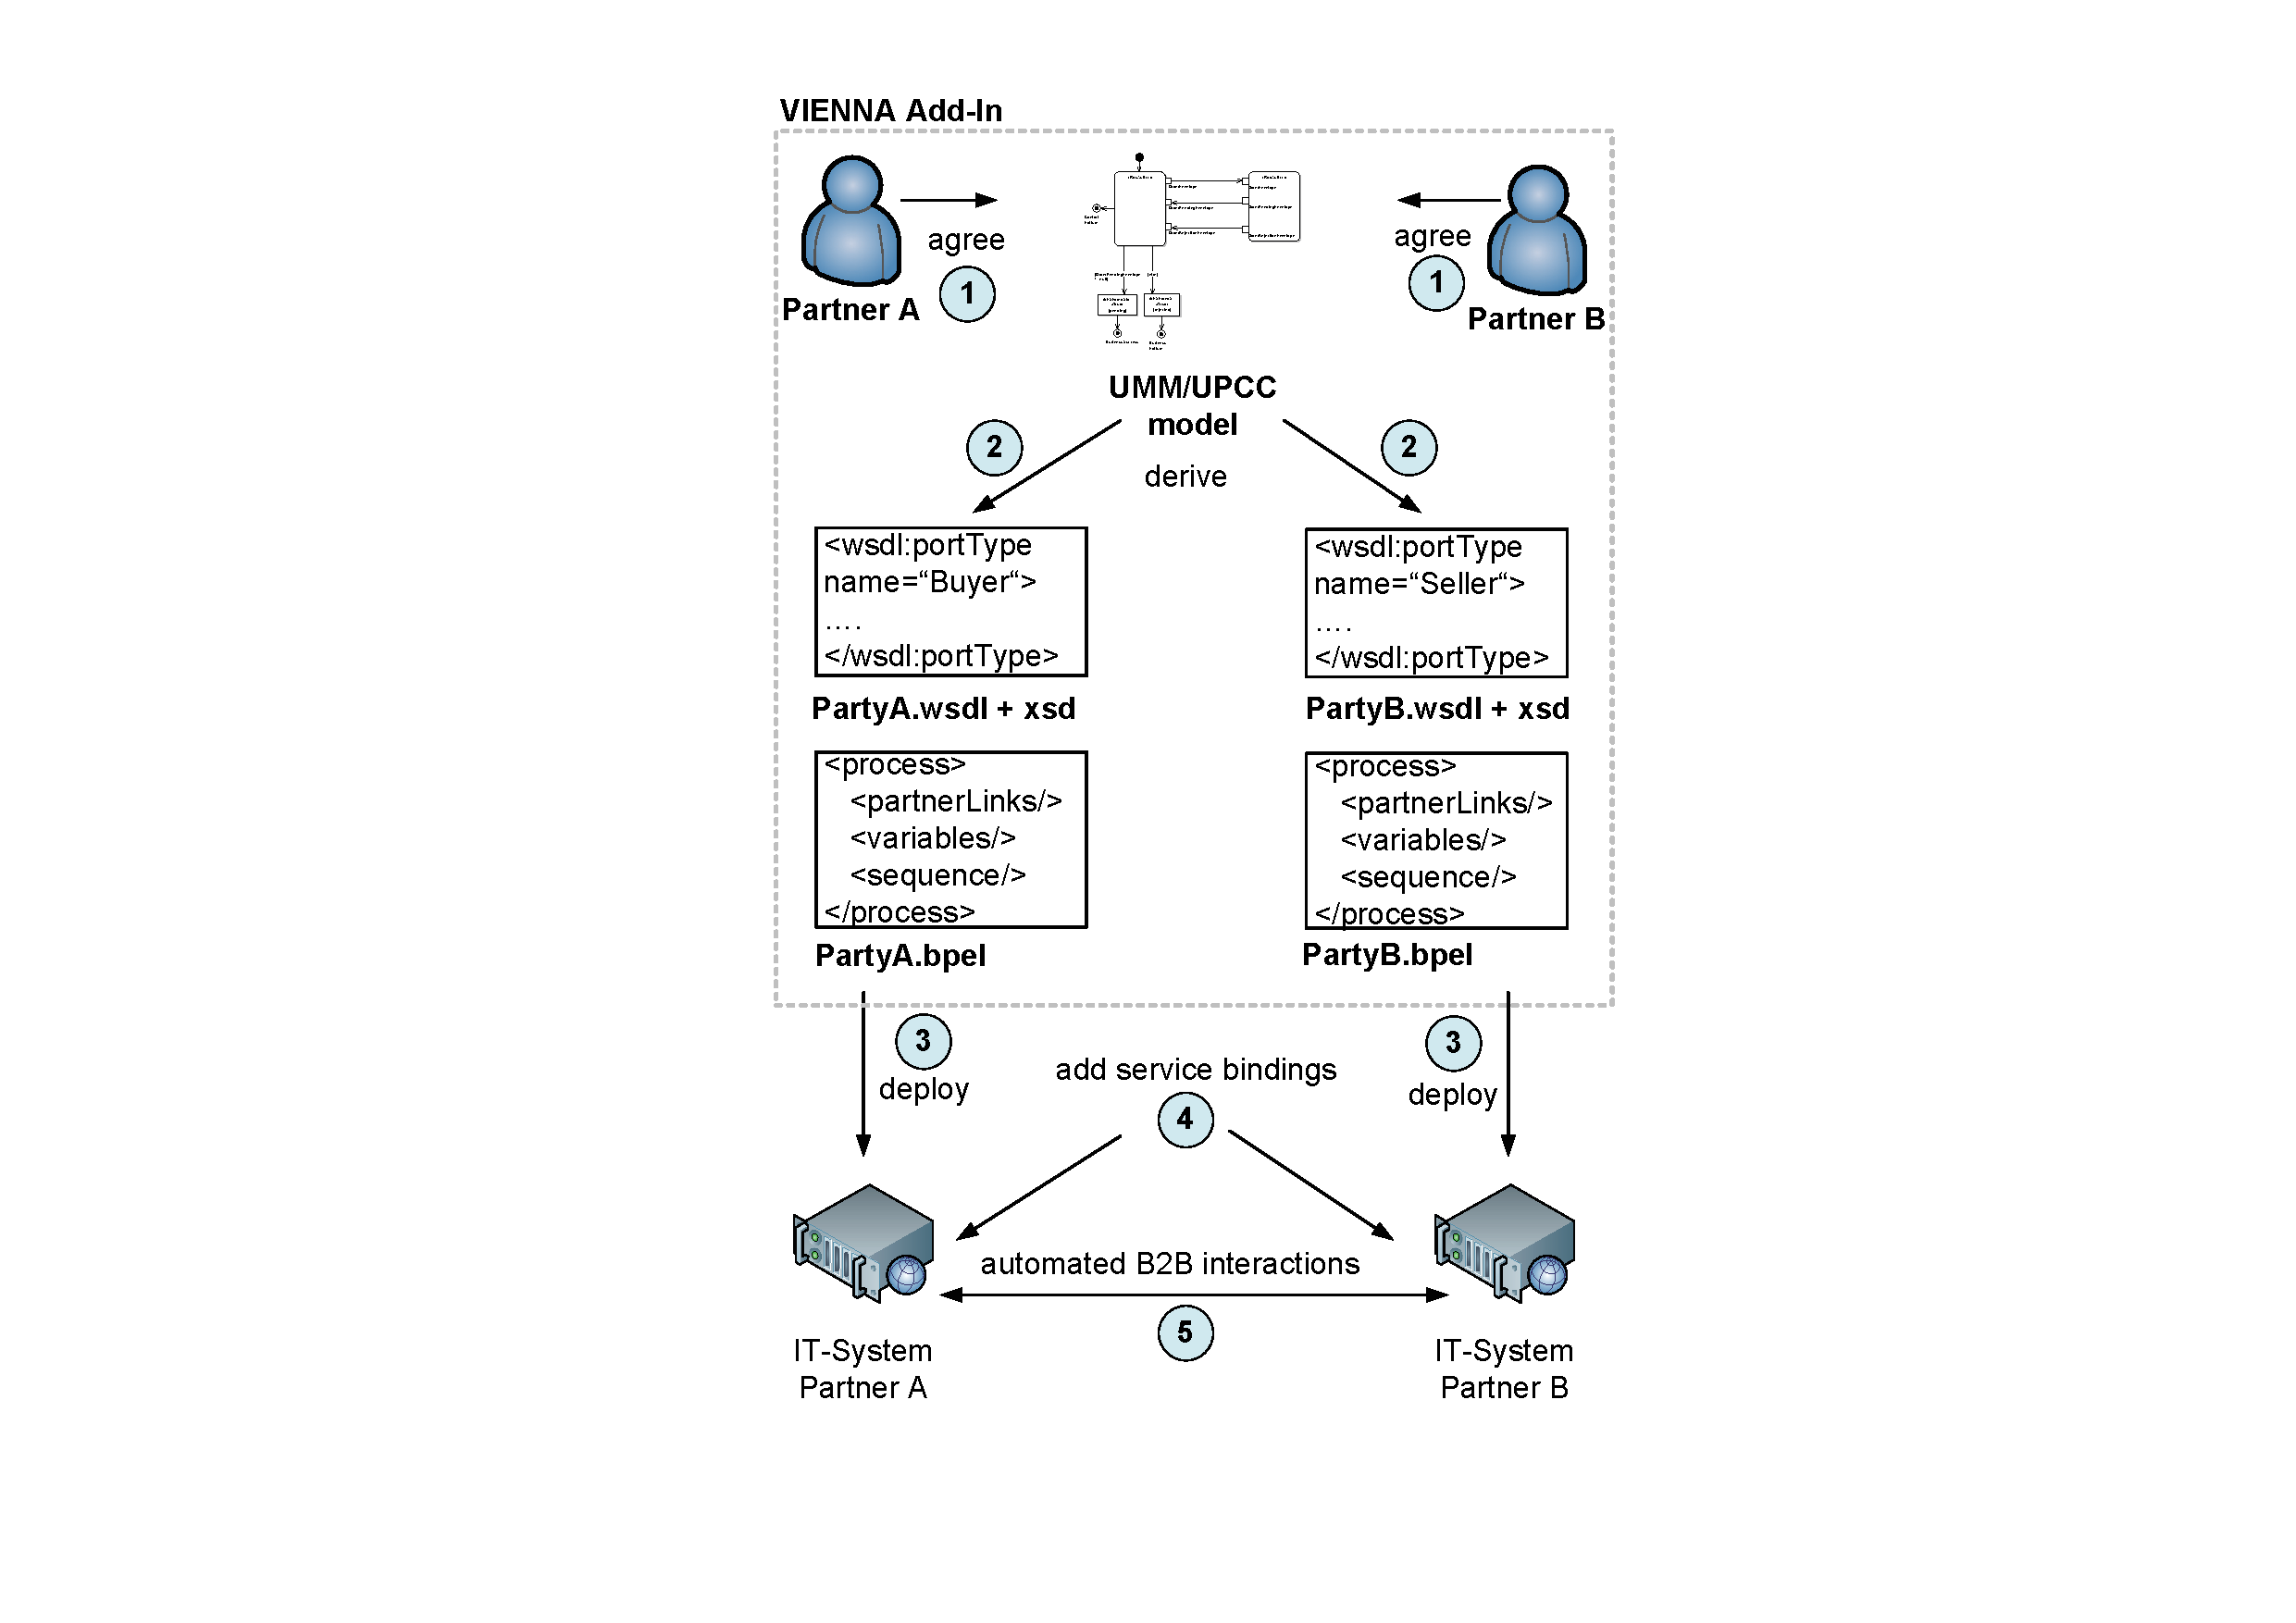
\includegraphics[width=0.37\textwidth]{figures/addinoverview.pdf}
 \caption{VIENNA Add-In overview}
 \label{fig:viennaaddinoverview}
\end{figure}


\section{UML Profile Definition} by TM

- explain the concepts of the MDG - the dynamic loading from umm-dev.org and the quicklinker

\section{Semi-automatic artifact generation} by CP und CE

explain the ABIE wizard and BDT wizard. rather concentrate on the facilitation benefit of the wizard than on the technical details behind it

\section{XML schema generation} by MS

explain the XSD generator - motivate the benefit of deriving schema from conceptual models




%Use the three references where appropriate - do not add additional references since we are short of space anyway
\nocite{man:umm2} 
\nocite{man:upcc} 
\nocite{man:VIENNAAddIn}





\bibliographystyle{abbrv}
\bibliography{references}  
\end{document}
